\section{Effectiveness of an Adaptive Learning Chatbot on Student's Learning Outcomes Based on Learning Styles \cite{kaiss2023}}
\label{sec:kaiss2023}

Sites populares de educação online como o Moodle são fontes de material para estudantes de diferentes experiências e necessidades acadêmicas. Entretanto, sem um acompanhamento apropriado, os usuários desses sites podem encontrar dificuldades em escolher os materiais apropriados para estudar, visto que eles podem oferecer uma ampla variedade de recursos \apud{kaiss2023}{udupi2016}. Assim, surge a necessidade de um sistema educacional adaptativo capaz de prover recursos pertinentes para o aprendizado dos alunos durante o processo educacional. Nesse sentido, no artigo, foi explorada a aplicação de uma ferramenta de conversação inteligente.

Sistemas educacionais adaptativos tiveram um aumento de popularidade e de influência com o passar das últimas décadas. Eles podem proporcionar instruções e recomendações de recursos educacionais com base nos diferentes níveis de conhecimento, interesses, objetivos e características pessoais dos usuários. Desse modo, para que os sistemas mencionados anteriormente possam operar adaptativamente com base nas individualidades dos seus usuários, uma direção de pesquisa que tem ganhado popularidade nos últimos tempos faz uso de estilos de aprendizado \apud{kaiss2023}{hasibuan2016}. Esses estilos de aprendizagem são formas predominantes pelas quais os alunos focam, processam, absorvem e retêm novas informações \apud{kaiss2023}{pashler2008}.

Modelos de estilos de aprendizado têm provado seu impacto na otimização do aprendizado acadêmico \apud{kaiss2023}{cruz2013}. No entanto, dadas as grandes mudanças e a liberdade da aquisição de conhecimento trazida pelo ensino online, teorias clássicas baseadas em ambientes tradicionais, sistemáticos e lineares de ensino podem não ser totalmente apropriadas para esse novo formato de ensino. Apesar de muitas pessoas ignorarem o fato de que o comportamento e o estilo de aprendizado dos estudantes variam da forma tradicional de ensino para o online, um crescente número de pesquisadores têm aplicado modelos de estilos de aprendizado no ensino online. Entretanto, a quantidade de estudos voltados para estilos online de aprendizado ainda é baixa, e na sua maioria, os modelos ainda estão na fase de criação.

Ao longo do tempo, diversos modelos de estilos de aprendizado foram propostos \apud{kaiss2023}{felder1988,honey1992,dunn1990,pask2011}. Para o desenvolvimento do sistema apresentado pelo artigo foi utilizado o modelo de Felder e Silverman (FSLSM). A escolha desse modelo se deu por conta de ser o modelo mais utilizado em sistemas educacionais, devido a ser possível quantificar o estilo de aprendizado dos alunos por meio dele. Além disso, para \apud{kaiss2023}{carver1999,garcia2007}, ele é considerado o modelo mais adequado a ser utilizado em sistemas educacionais adaptativos, ao passo de também ser de fácil implementação \apud{kaiss2023}{lu2007,hwang2013}.

O modelo FSLSM adotado caracteriza o estilo de aprendizado de cada aluno ao longo de quatro dimensões. A dimensão de processamento (Ativa/Reflexiva), diz respeito ao processamento da informação. Um estudante ativo prefere trabalhar em grupo e experimentar mais, já um estudante reflexivo prefere refletir, seja sozinho ou com uma companhia familiar. A dimensão de recepção (Visual/Verbal) é destinada à apresentação da informação. Um aluno visual gosta mais de apresentações visuais como imagens, diagramas e fluxogramas, já um aluno verbal tende a escolher apresentações orais e textuais. A dimensão de entendimento (Sequencial/Global) está relacionada à forma de organizar e progredir na compreensão da informação. Um estudante sequencial pensa de forma linear e aprende de formal incremental por meio de pequenos passos, em contraste do estudante global, que têm um pensamento sistemático e aprende em grandes saltos. A dimensão de percepção (Sensitiva/Intuitiva) trabalha sobre a percepção e assimilação da informação. Um aluno sensitivo possui um pensamento concreto, além de ser prático e compromissado com fatos e procedimentos, em contrapartida do aluno intuitivo, que é adepto da inovação e do pensamento conceitual.

Como parte do modelo FSLSM, também há um questionário composto de 44 perguntas que são usadas para determinar o estilo de aprendizado de cada aluno com base nas respostas fornecidas a ele. Assim, é possível classificar de maneira prévia cada estudante antes de eles usarem de fato um sistema adaptativo, resolvendo assim alguma problemática que aconteceria caso eles utilizassem o sistema sem que houvesse nenhuma informação sobre o estilo de aprendizado que eles possuem.

Como proposta de sistema educacional adaptativo, no artigo é desenvolvido um chatbot chamado \textit{LearningPartnerBot}, que possui a capacidade de recomendar em tempo real recursos educacionais, com base no estilo de aprendizado de cada aluno. Pensando na facilidade do acesso dos discentes a esse chatbot, ele foi construído sobre a plataforma Moodle, devido a ela ser uma das mais utilizadas na internet, além de estar disponível em uma ampla variedade de dispositivos, e de ser facilmente adaptável e extensível.

Na Figura \ref{fig:architecture-kaiss}, é apresentada a arquitetura da abordagem explorada como sistema educacional adaptativo. Conforme mencionado anteriormente, para os novos usuários da plataforma, é aplicado o questionário do modelo FSLSM com o intuito de classificar seu estilo de aprendizado preferido. Após isso, o resultado é persistido em uma base de dados dedicada aos dados dos alunos, que será consumida por um módulo do sistema responsável por recomendar recursos educacionais com base na preferência do usuário. E nesse contexto, a interação do discente com esse módulo de recomendação é intermediada pelo chatbot \textit{LearningPartnerBot} integrado na plataforma Moodle. Vale ressaltar que, para o processamento de linguagem natural das mensagens enviadas para o chatbot pelos alunos, é utilizada uma versão de código aberto do Framework DialogFlow da Google, que permite que as solicitações em linguagem natural sejam convertidas em um formato computacionalmente legível para o módulo de recomendações.

\begin{figure}[ht] 
   	\captionsetup{width=16cm}
	\Caption{\label{fig:architecture-kaiss} Arquitetura do sistema adaptativo desenvolvido}
	\UFCfig{}{
        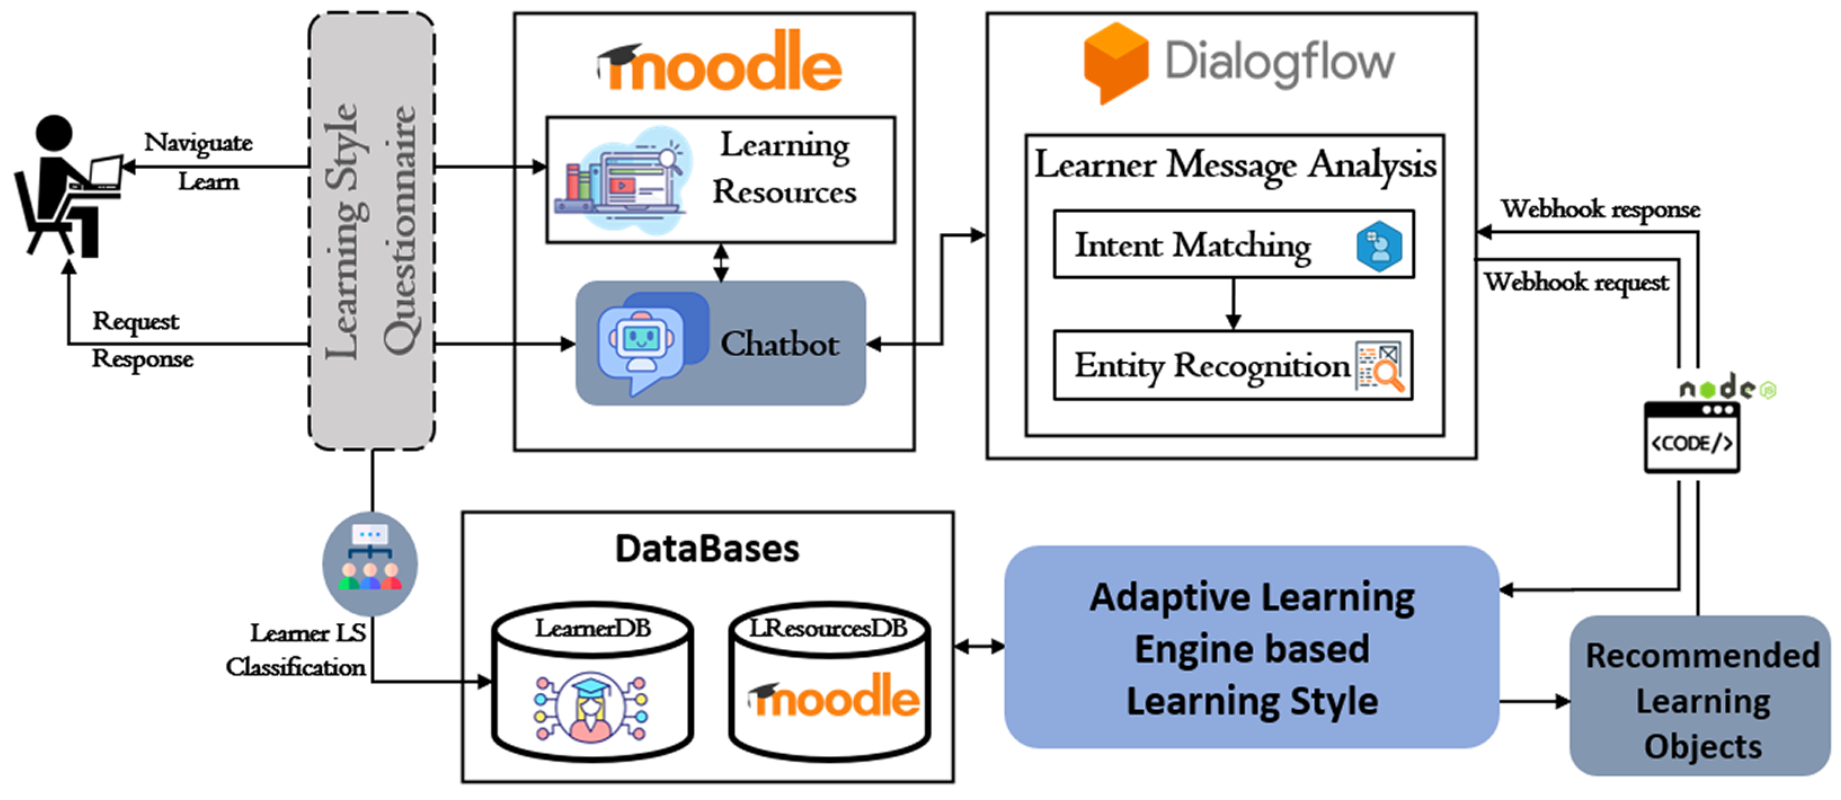
\includegraphics[width=16cm]{figuras/architecture-kaiss.png}
    }{
		\Fonte{\citeonline{kaiss2023}.}
	}
\end{figure}

Na fase de experimentação, a abordagem desenvolvida foi aplicada em uma disciplina de programação em linguagem C, para alunos do primeiro ano dos cursos de Software Engineering and Distributed Computing Systems (GLSID) e Big Data and Cloud Computing Engineering (BDCC) da escola de ensino superior marroquina Ecole Normale Supérieure de l’Enseignement Technique de Mohammedia (ENSET). A população total do estudo era de 71 discentes (Sendo 52 homens e 19 mulheres), na faixa etária de 20 a 21 anos. Durante essa etapa, os estudantes puderam usar o chatbot livremente pelo período de duas semanas e no dispositivo de sua preferência.

Na Figura \ref{fig:visual-style-recommendations-kaiss}, é mostrado um exemplo de recomendação de recurso educacional para caso o aluno tenha um estilo de aprendizado visual, em que por exemplo, ao clicar em um dos materiais fornecidos, ele será redirecionado para um conteúdo em formato de vídeo. Já no exemplo da Figura \ref{fig:verbal-style-recommendations-kaiss}, são apresentadas recomendações para caso o aluno possua um estilo textual, em que os recursos recomendados estão na forma de texto, de documentos em PDF e de apresentações em slides. A lista de recomendações dadas pelo chatbot são sempre clicáveis para facilitar o redirecionamento e a pesquisa dentro do Moodle.

\begin{figure}[ht] 
   	\captionsetup{width=16cm}
	\Caption{\label{fig:visual-style-recommendations-kaiss} Exemplo de recomendação para o estilo de aprendizado visual}
	\UFCfig{}{
        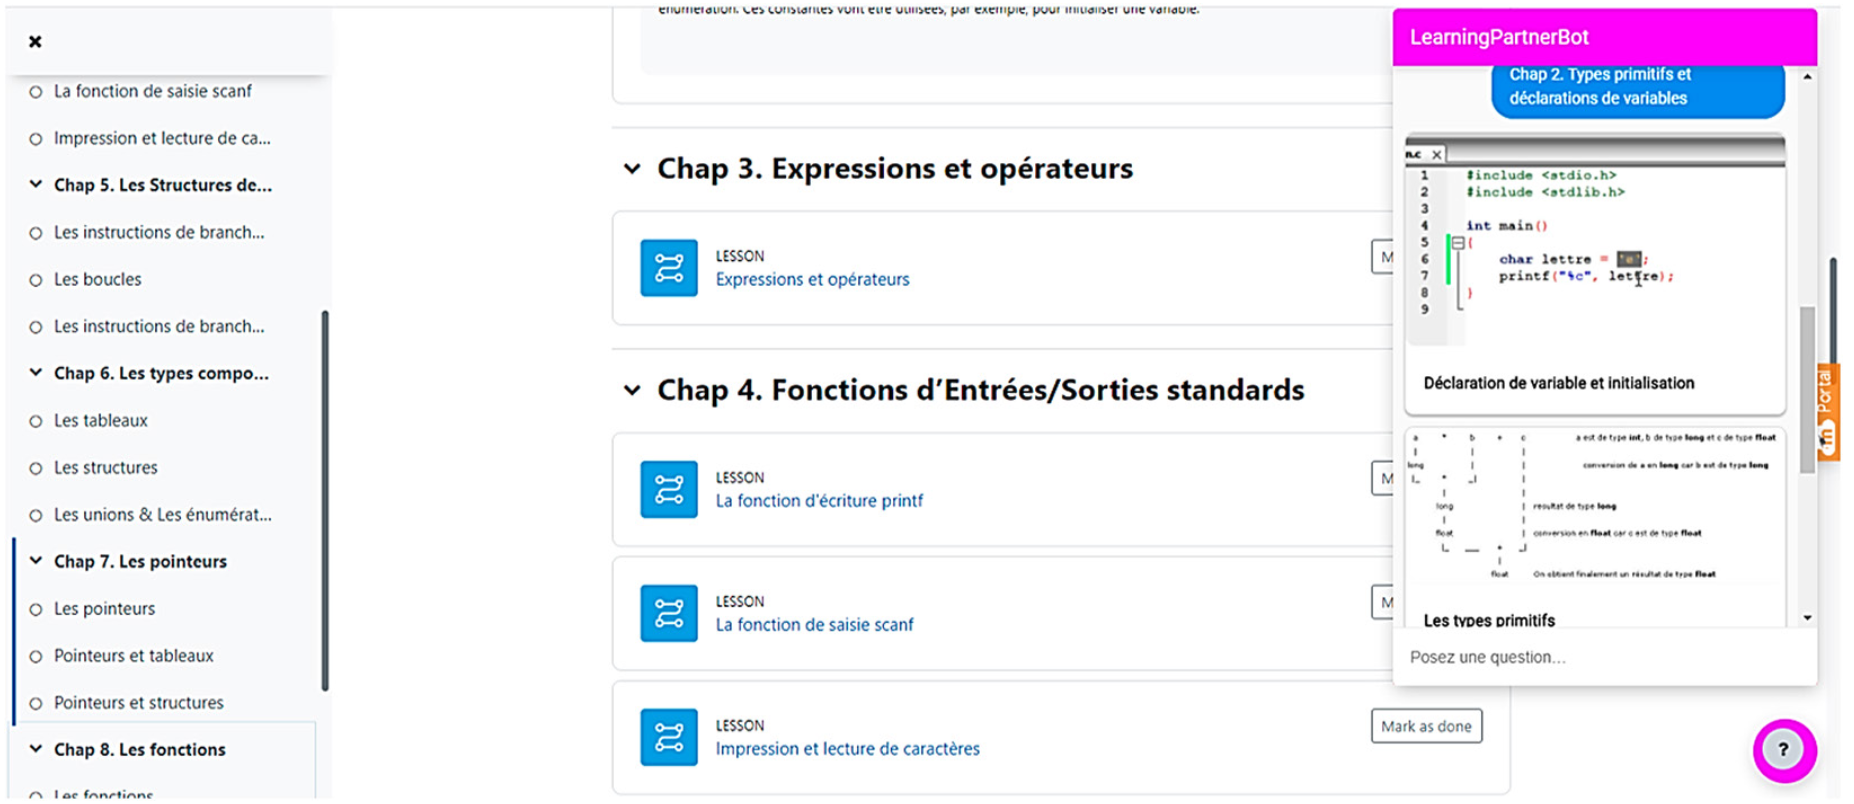
\includegraphics[width=16cm]{figuras/visual-style-recommendations-kaiss.png}
    }{
		\Fonte{\citeonline{kaiss2023}.}
	}
\end{figure}

\begin{figure}[ht] 
   	\captionsetup{width=16cm}
	\Caption{\label{fig:verbal-style-recommendations-kaiss} Exemplo de recomendação para o estilo de aprendizado textual}
	\UFCfig{}{
        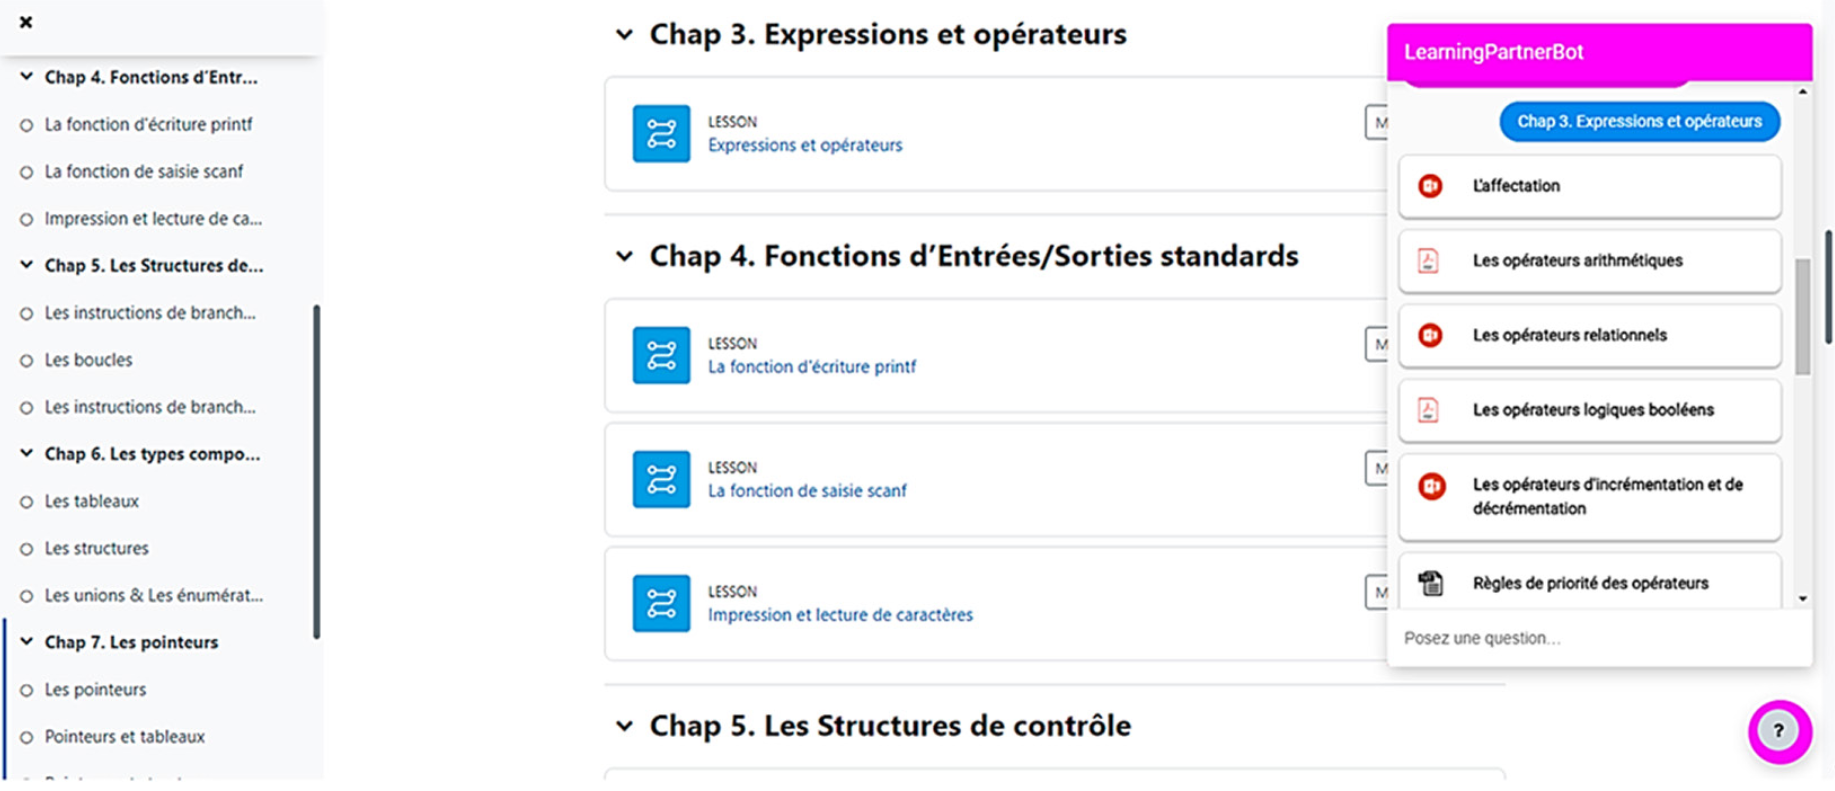
\includegraphics[width=16cm]{figuras/verbal-style-recommendations-kaiss.png}
    }{
		\Fonte{\citeonline{kaiss2023}.}
	}
\end{figure}

Antes do uso do chatbot pelos alunos, foi aplicado um pré-teste com o intuito de avaliar o nível de conhecimento que eles possuíam antes do experimento. Esse teste mostrou que 61\% deles estavam no nível iniciante e 39\% no nível intermediário. No pós-teste, os resultados obtidos mostraram que 45\% dos estudantes continuaram no nível iniciante, 49\% no intermediário e 6\% no avançado. Na Figura \ref{fig:results-kaiss}, é feito um comparativo dos dados obtidos, onde é possível perceber que a quantidade de alunos no nível iniciante teve uma diminuição de 16\%, ao passo que no nível intermediário teve um aumento de 10\%, além de que, também apareceram alunos considerados de nível avançado (6\%).

\begin{figure}[ht] 
   	\captionsetup{width=16cm}
	\Caption{\label{fig:results-kaiss} Comparação dos resultados entre o pré e o pós teste dos participantes}
	\UFCfig{}{
        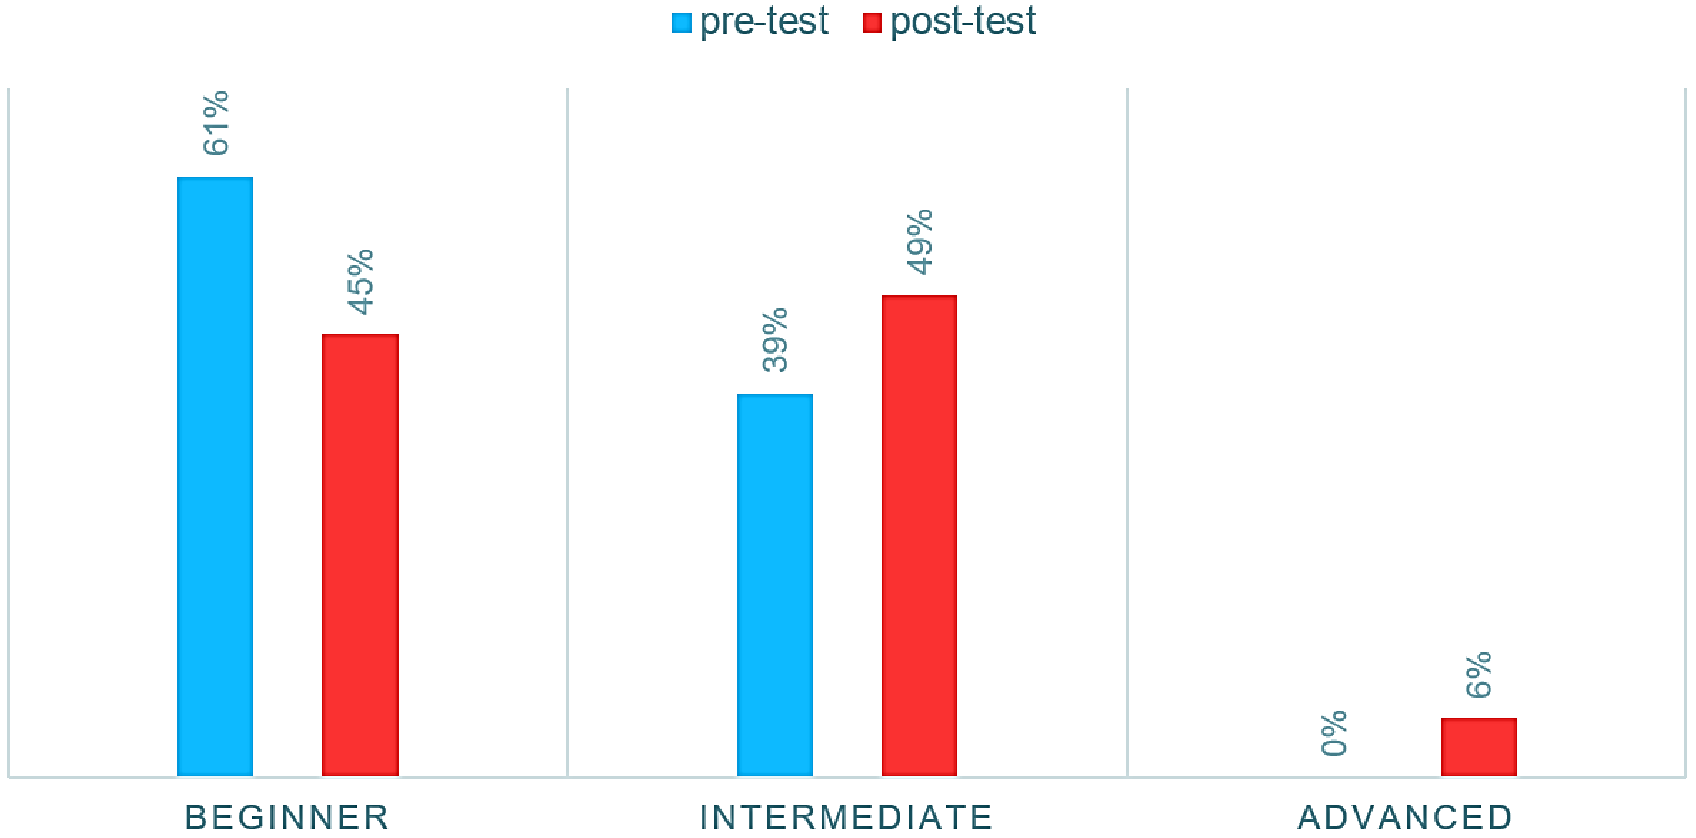
\includegraphics[width=16cm]{figuras/results-kaiss.png}
    }{
		\Fonte{\citeonline{kaiss2023}.}
	}
\end{figure}

Por fim, para avaliar a satisfação dos participantes da pesquisa em relação à abordagem proposta, após o pós-teste, foram feitas a eles as seguintes perguntas: "As recomendações apresentadas pelo \textit{LearningPartnerBot} foram úteis no processo de aprendizado?" e "Como você classifica a sua experiência geral utilizando o \textit{LearningPartnerBot}?". Os resultados coletados por essas perguntas estão apresentados na Tabela \ref{tab:results-kaiss}, que mostra a alta satisfação que os discentes tiveram com o uso do sistema educacional adaptativo construído.

\begin{table}[ht]
	\captionsetup{width=13cm}
	\Caption{\label{tab:results-kaiss} Satisfação dos participantes em relação à abordagem proposta}
	\IBGEtab{}{
		\begin{tabular}{lrrr}
			\toprule
            & Pouco interessante & Interessante & Muito interessante \\
			\midrule
			Satisfação das recomendações & 2\% & 25\% & 73\% \\
			Satisfação do uso do chatbot & 0\% & 9\% & 91\% \\
			\bottomrule
		\end{tabular}
	}{
	\Fonte{\citeonline{kaiss2023}}
}
\end{table}